\documentclass{article}
\usepackage{amsmath}
\usepackage{amssymb}
\usepackage{graphicx}
\usepackage{hyperref}
\usepackage[version=4]{mhchem}


\begin{document}
In parallelogram \(A B C D\), point \(E\) is the midpoint of \(A B\), and point \(F\) is on \(A D\) so that \(\frac{A F}{A D}=\frac{1}{3}\). Let \(G\) be the point of intersection of \(A C\) and \(F E\). Find \(\frac{A C}{A G}\).\\
\centering
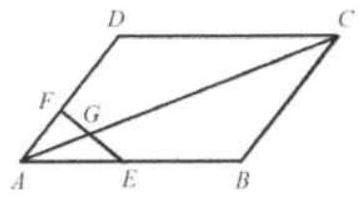
\includegraphics[width=\textwidth]{images/123.jpg}

Solution: 5.
Extend \(F E\) through \(E\) to \(H\) and to meet the extension of \(C B\) at \(H\).\\
We know that \(A D / / C H\). So \(\triangle A E F \sim \triangle B E H\) (Figure 1). \(\frac{A F}{B H}=\frac{A E}{E B} \quad \Rightarrow B H=A F\). So we know that \(C H=C B\) \(+B H=A D+A F=4 A F\).\\
\centering
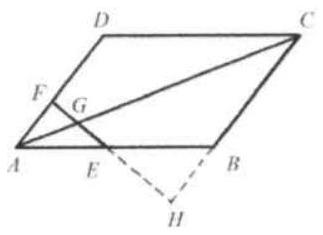
\includegraphics[width=\textwidth]{images/123(1).jpg}

We know that \(A F / / C H\). So \(\triangle A G F \sim \triangle C G H\) (Figure 2). \(\frac{A F}{C H}=\frac{A G}{G C} \Rightarrow\)

\[
\begin{aligned}
& \frac{A F}{4 A F}=\frac{A G}{G C}=\frac{1}{4} \quad \Rightarrow \quad \frac{G C}{A G}=4 \quad \Rightarrow \quad \frac{A C-A G}{A G}=4 \Rightarrow \\
& \frac{A C}{A G}-1=4 \quad \Rightarrow \quad \frac{A C}{A G}=5 .
\end{aligned}
\]

\begin{center}
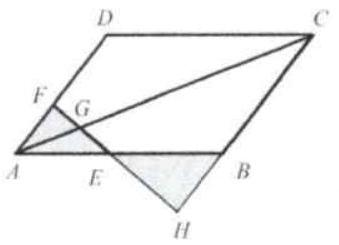
\includegraphics[width=\textwidth]{images/124.jpg}
\end{center}

Figure 1\\
\centering
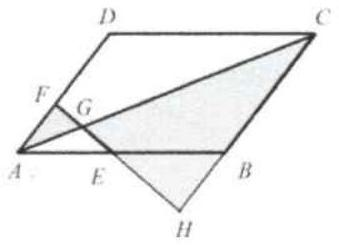
\includegraphics[width=\textwidth]{images/124(2).jpg}

Figure 2


\end{document}
